\subsection{Iteration 2: Zambia Coach Training}

This time, the iteration has a more detailed scope, with a hypothesis on what needs the app should meet in the end, and create lo-fi and hi-fi trigger material to meet those needs.

A co-creation workshop started the interactions, followed by repeated app tests at minimum one session per day, always followed by a feedback round, so the app and the tomorrow's question set creation could be improved for the next day. At the end of the week, there was a co-refinement workshop of the current hi-fi material, and also lo-fi material for the new version of the app.

\subsubsection*{Creation of questions}
Project leader Josefina in Zambia refined Iliana's first question sets, prepared for the visit to Zambia. Josefina created question sets with Bloom at the back of her head, also taking into account the structure and the order of the coach manuals, what it means being a coach within the topic, and lastly scenarios.

\subsubsection{Trigger material used}
A hi-fi trigger material was done, a very basic quiz app, keeping it as simple as possible (see Application Implementation, Iteration 2). All of the devices (tablets and smartphones) that were kept in Kampala were brought to Zambia. Josefina's questions were added to the app, and the app was installed on all of the devices. This process was repeated for all the days, Sunday-Friday.

\subsubsection{Design workshop \#1 in Zambia}
The coach training started with having a design workshop with the coaches, see figure \ref{fig:zambia}, not showing them the hi-fi trigger material yet. The co-creation workshop was made to let the coaches create a lo-fi prototype, and as a result identify important functionality in the minds of the coaches.

\begin{enumerate}
\item Since the knowledge about smartphones and apps were low, an introducing to topics was made.
\item All were familiar with what Facebook was, so thus the Facebook app was shown as an example. Wanting to know what the app would look like if the coaches would have designed the app, they were trained how to design an app via drawing wireframes.
\item Using postits, they started with during limited time drawing the start view from the Facebook app.
\item Then, they were asked to draw what they thought happened on the friend icon click, drawing the view on another postit.
\item Then, the mission of the YoungDrive app was described. They were then divided into two teams, having limited time to draw the best imaginable YoungDrive coach quiz app they could. First, they designed the app from the top of their heads. They then pitched their results to each other.
\item On the next iteration, they were to suggest and design improvements how the app should be designed to improve learning, not only assessment. They then again pitched their results to each other.
\end{enumerate}

\begin{figure}[h]
    \centering
    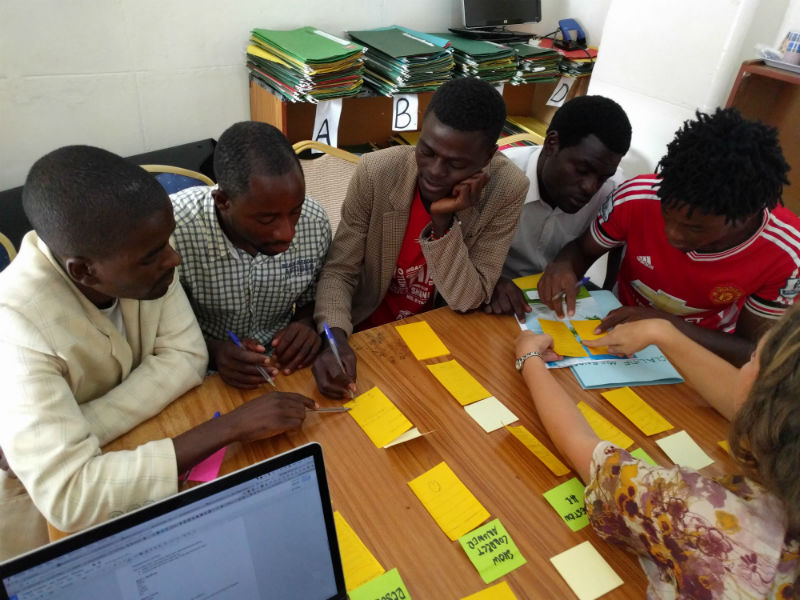
\includegraphics[width=0.7\textwidth]{zambiaCreation.jpg}
    \caption{Each person designed a YoungDrive app first for assessment, then adapting the app for learning. They were allowed to test the smartphones and tablets, and use the apps Quizoid or Duolingo for reference.}
    \label{fig:iteration}
\end{figure}

\subsubsection{Assessment via quiz}
At the end of each day, the app was used to test the coaches' knowledge. Each coach got either a smartphone, tablet or computer. The coach first took the quiz for the most recent session, and could then choose what to do next.

As there were no back-end developed, Josefina by hand documented the scores of each coach, writing the name of the coach, the session, number of correct answers, and what questions had been answered wrong.

Josefina then, when planning the next day, looked at the statistics, looking for trends that would inform the sessions for the following day. She also evaluated the quality of the questions, before creating the new question sets for the next day.

\subsubsection{Experimenting with quiz before or after the session}
Since the coaches appreciated the app so much, we felt tempted to try what would happen with fun and learning if we tried using the app \textit{before} a session instead of only after. During the rest of the week, we continued, finally finding preferences and tendencies from the coaches, via observation, interviews, and survey.

\subsubsection{Experimenting with design of questions}
During the week, extra tests were done to test the following:

\begin{itemize}
\item Number of questions per quiz
\item Single-answer questions or multiple-answer questions
\item Framing of questions
\item Challenge level of questions
\item Determining what made a question hard
\end{itemize}

\subsubsection{Interviews with Josefina}
At the end of each day, an evaluation interview was held with Josefina. At the end of the week, a final interview was held. At the end of Day 5, a discussed was made with Josefina what it would look like to not record the answers manually, but pushing the results online. A co-creation workshop was held, where she drew an Educator Dashboard.

\subsubsection{Design workshop \#2 in Zambia}
In the last day of training, another workshop was held, where the question was: "What do you need in order to feel self-confident for your session?". This question was informed from iteration 1. The coaches was asked to write down one need per post-it during limited time, then choosing the most important need, and then writing a motivation why that need was important to them. Finally, they were asked to sketch what an app would look like, that addressed this need to them.
